\section{Application}
\subsection{Présentation:}

\subsubsection{IHM}
L'application contient principalement cinq écrans:
\paragraph{La page d'accueil(fig.\ref{fig:page_home}): } Cette page contient des élements suivants:
\begin{itemize}
  \item Un bar de recherche qui ramène à la page recherche;
  \item Un modal(fig.\ref{fig:modal_setting}) pour la configuration personnalisée;
  \item Des buttons comme accès rapide vers la page recherche.
\end{itemize}

\begin{figure}[h]
\centering
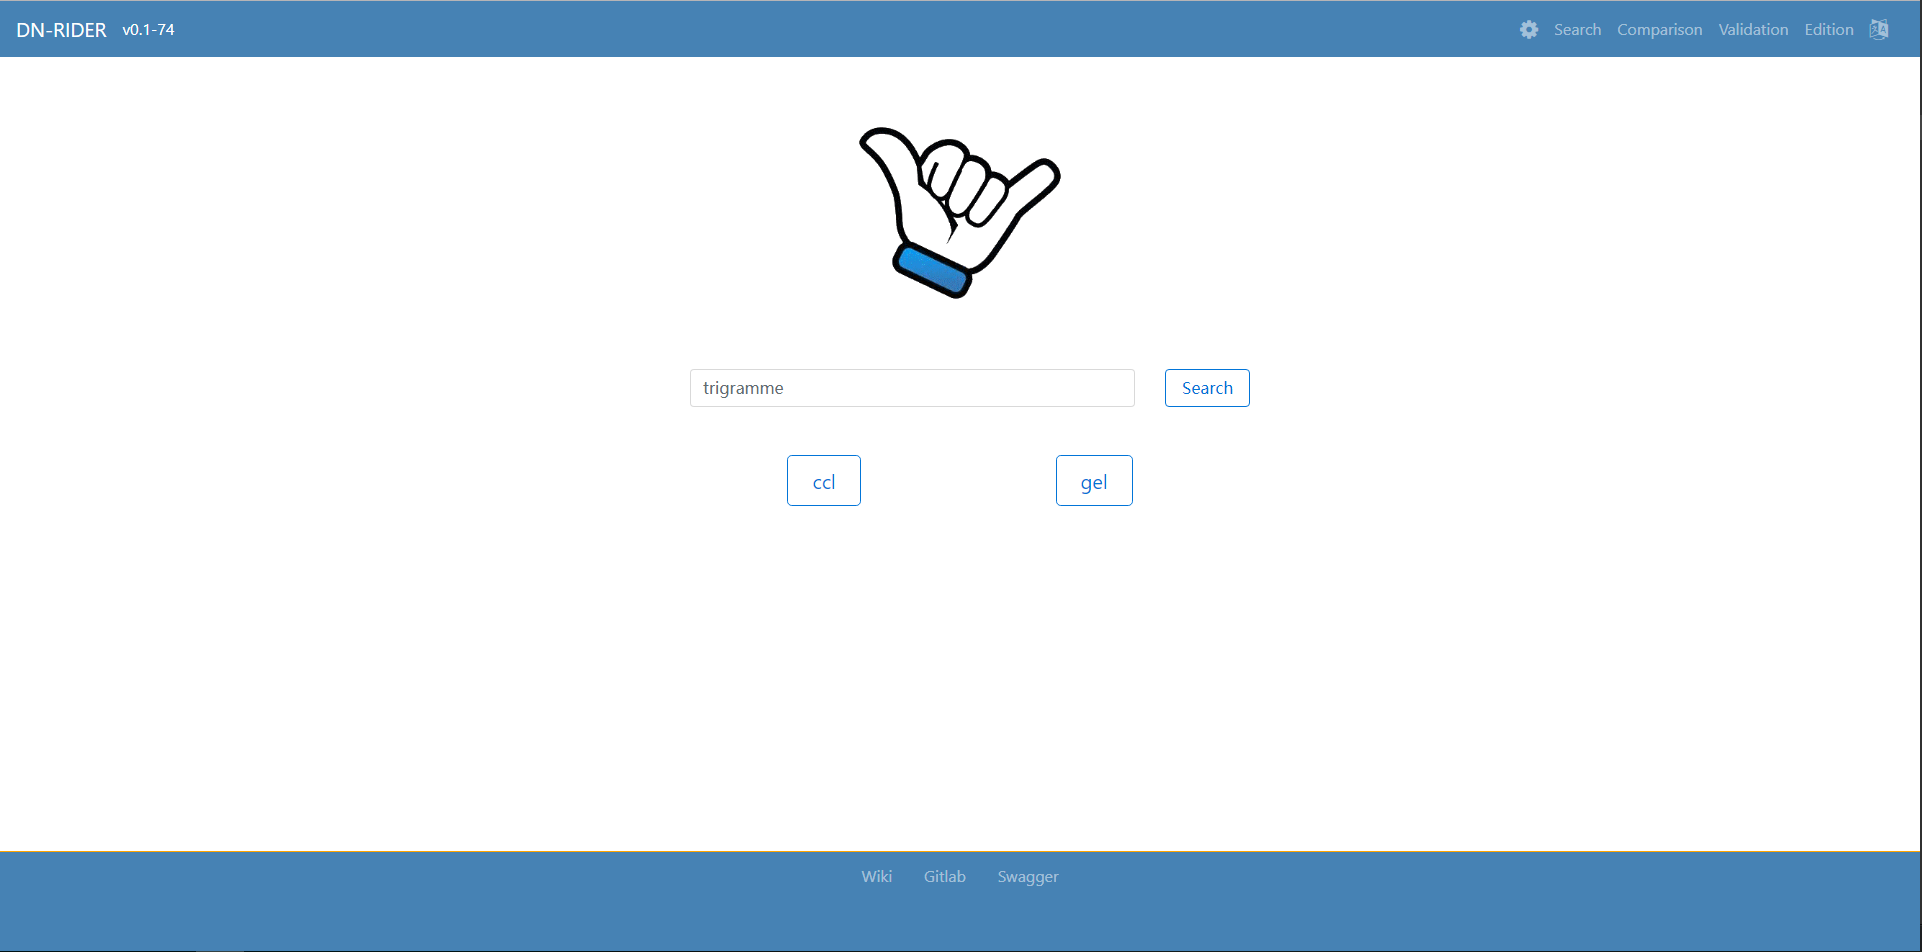
\includegraphics[width=0.8\textwidth]{page_home}
\caption{La page d'accueil}
\label{fig:page_home}
\end{figure}

\begin{figure}[h]
\centering
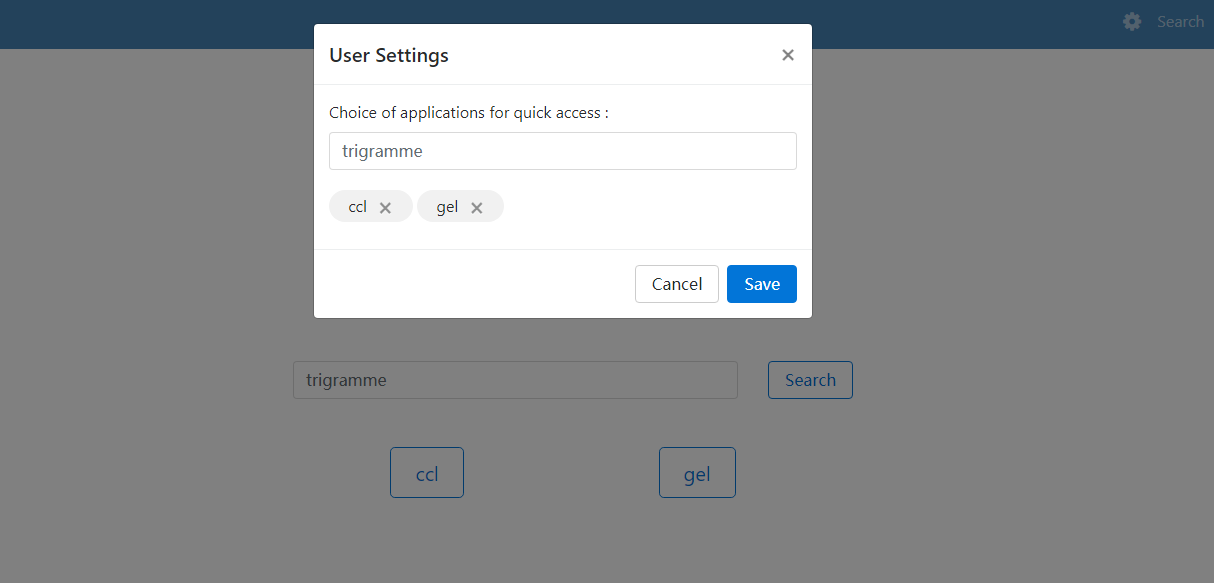
\includegraphics[width=0.6\textwidth]{modal_setting}
\caption{Le modal configuration}
\label{fig:modal_setting}
\end{figure}

\paragraph{La page recherche(fig.\ref{fig:page_search}): } Cette page contient des élements suivants:
\begin{itemize}
  \item Un sidebar collapsible qui contient un formulaire pour choisir les notes de livraisons;
  \item Une note de livraison au format json manipulative;
  \item Des buttons qui permet de swicher le format d'affichage et des liens vers la page validation et l'application Nexus.
\end{itemize}

\begin{figure}[h]
\centering
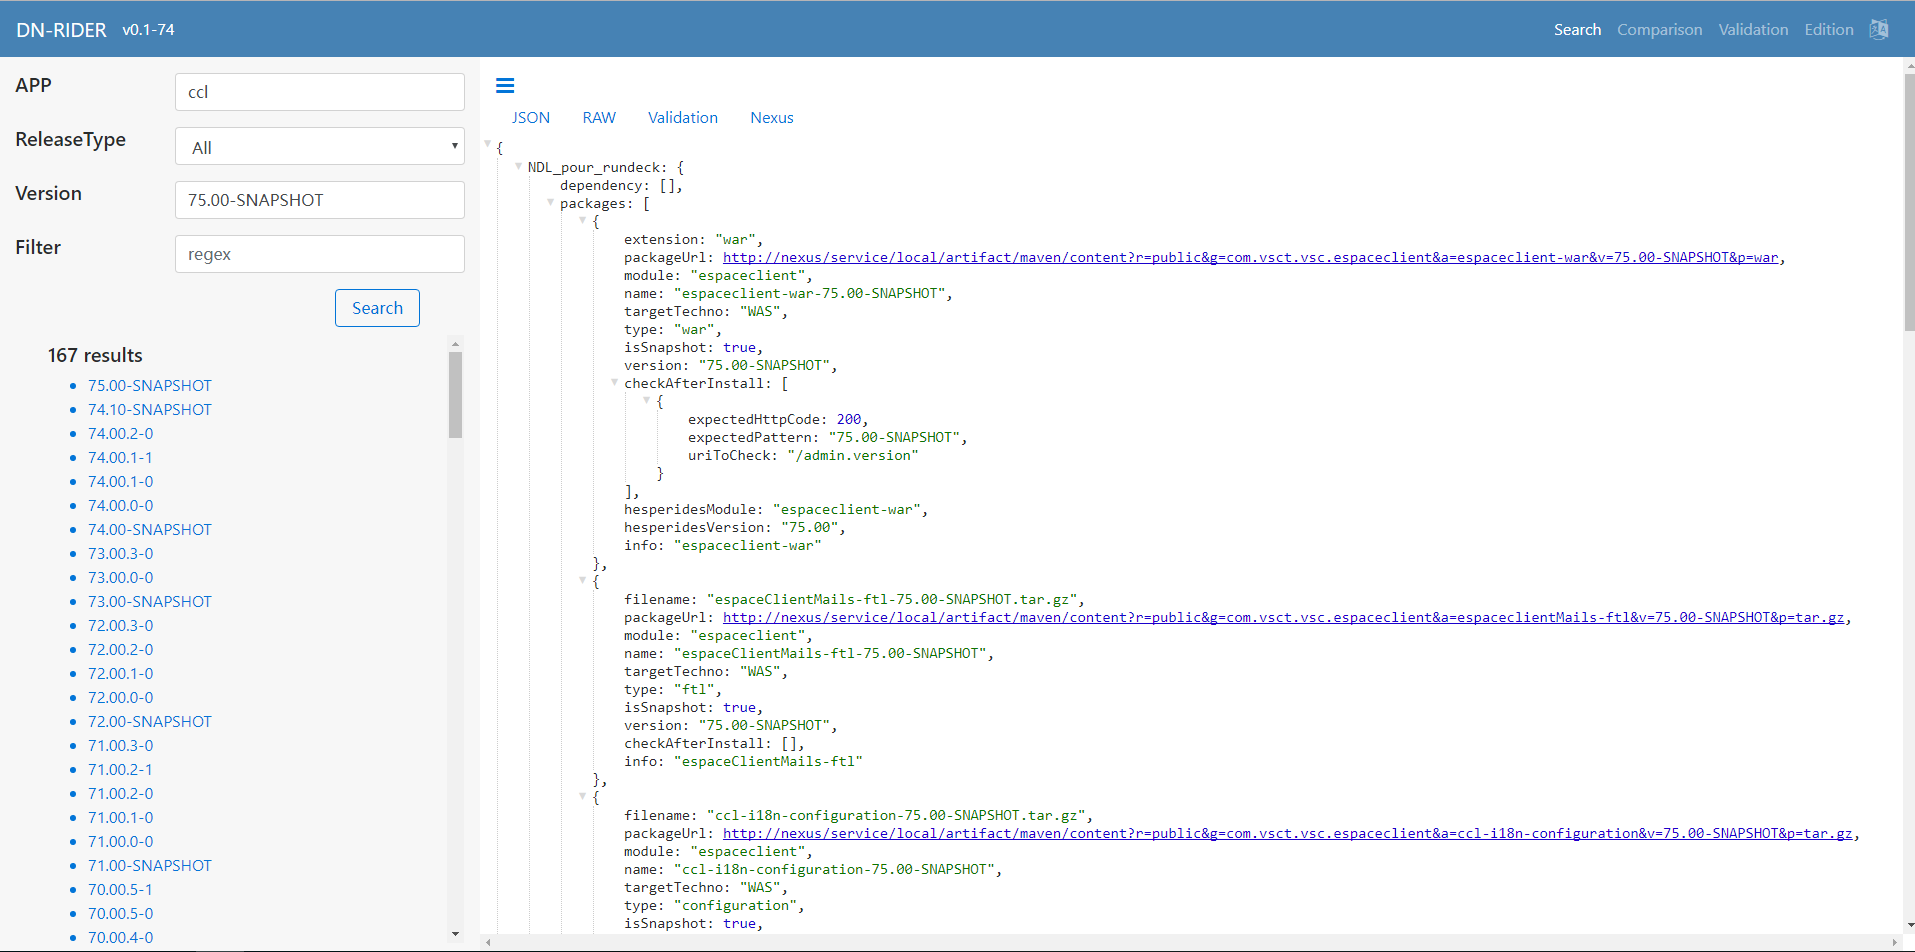
\includegraphics[width=0.8\textwidth]{page_search}
\caption{La page recherche}
\label{fig:page_search}
\end{figure}

\paragraph{La page validation(fig.\ref{fig:page_comparaison}): } Cette page contient des élements suivants:
\begin{itemize}
  \item Un sidebar collapsible qui contient un formulaire pour choisir les notes de livraisons;
  \item Un tableau qui compare les packages des notes de livraisons, le contenu des packages se présent dans un popover sous format json manipulatif;
\end{itemize}

\begin{figure}[h]
\centering
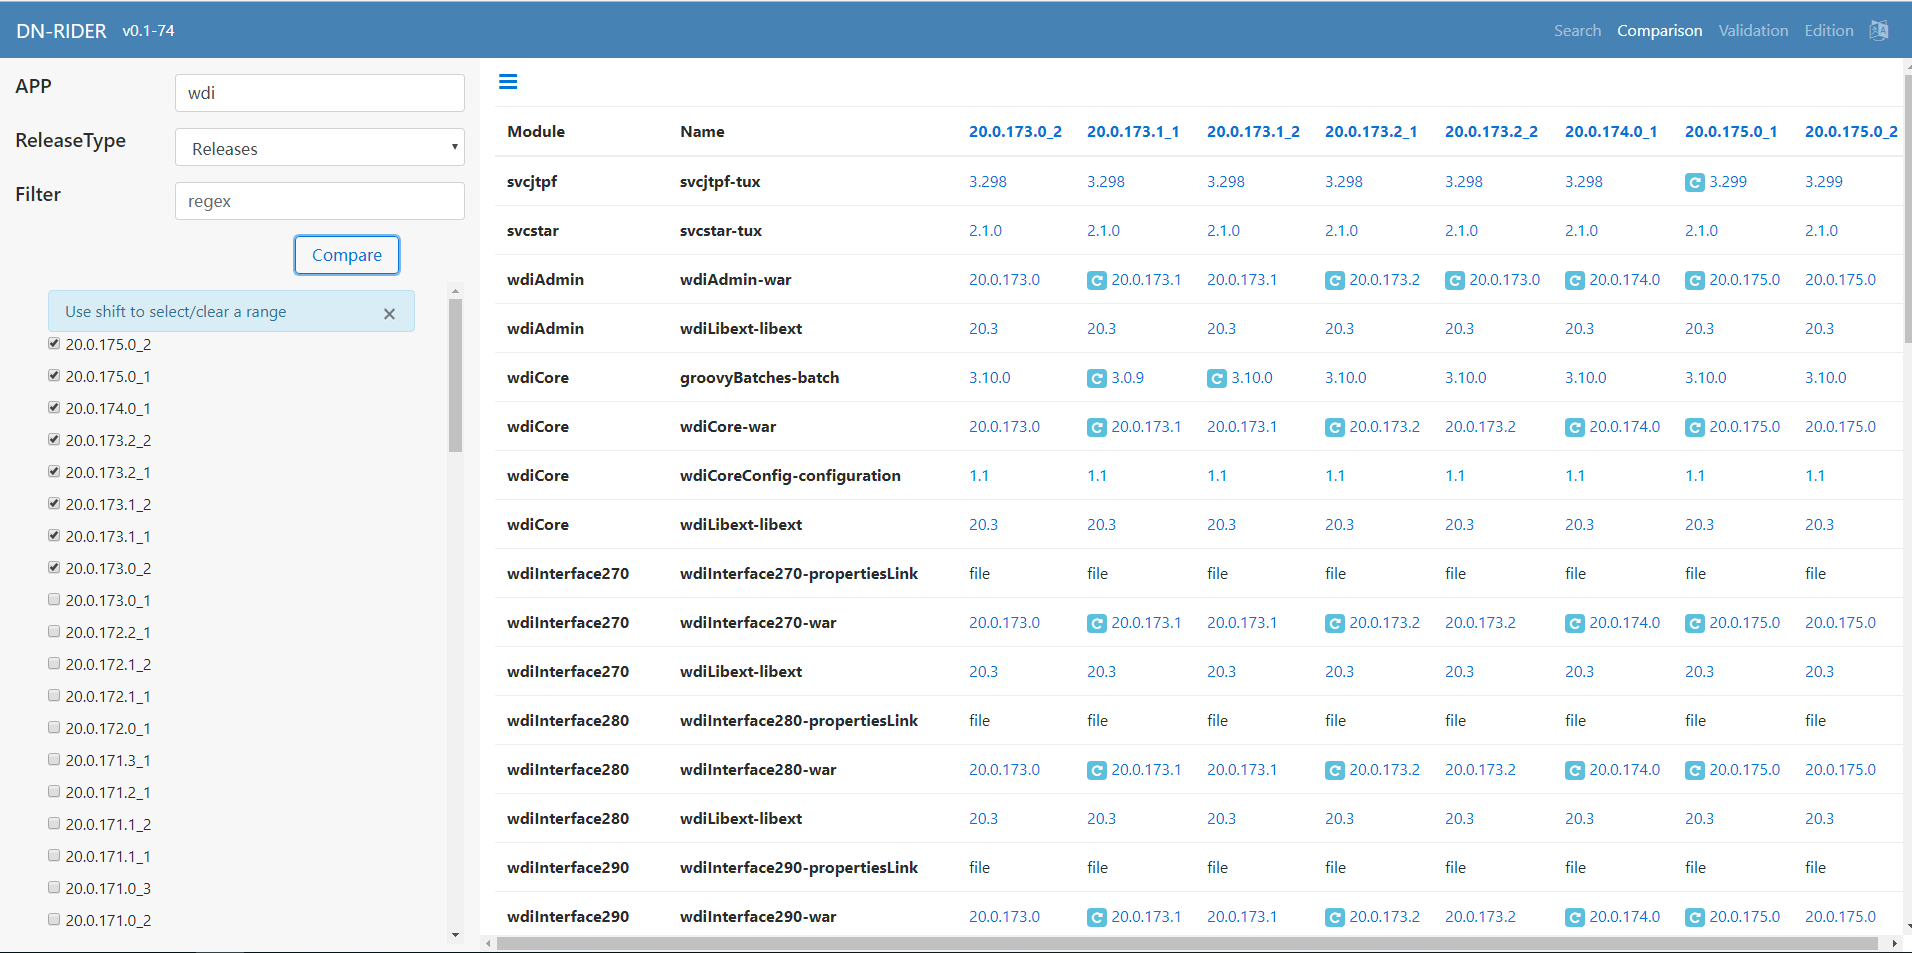
\includegraphics[width=0.8\textwidth]{page_comparison}
\caption{La page comparaison}
\label{fig:page_comparaison}
\end{figure}

\paragraph{La page validation(fig.\ref{fig:page_validation}): } Cette page contient des élements suivants:
\begin{itemize}
  \item Une zone qui permet d'éditer une note de livraison;
  \item Une fênetre qui affiche les résultats de validation;
\end{itemize}

\begin{figure}[h]
\centering
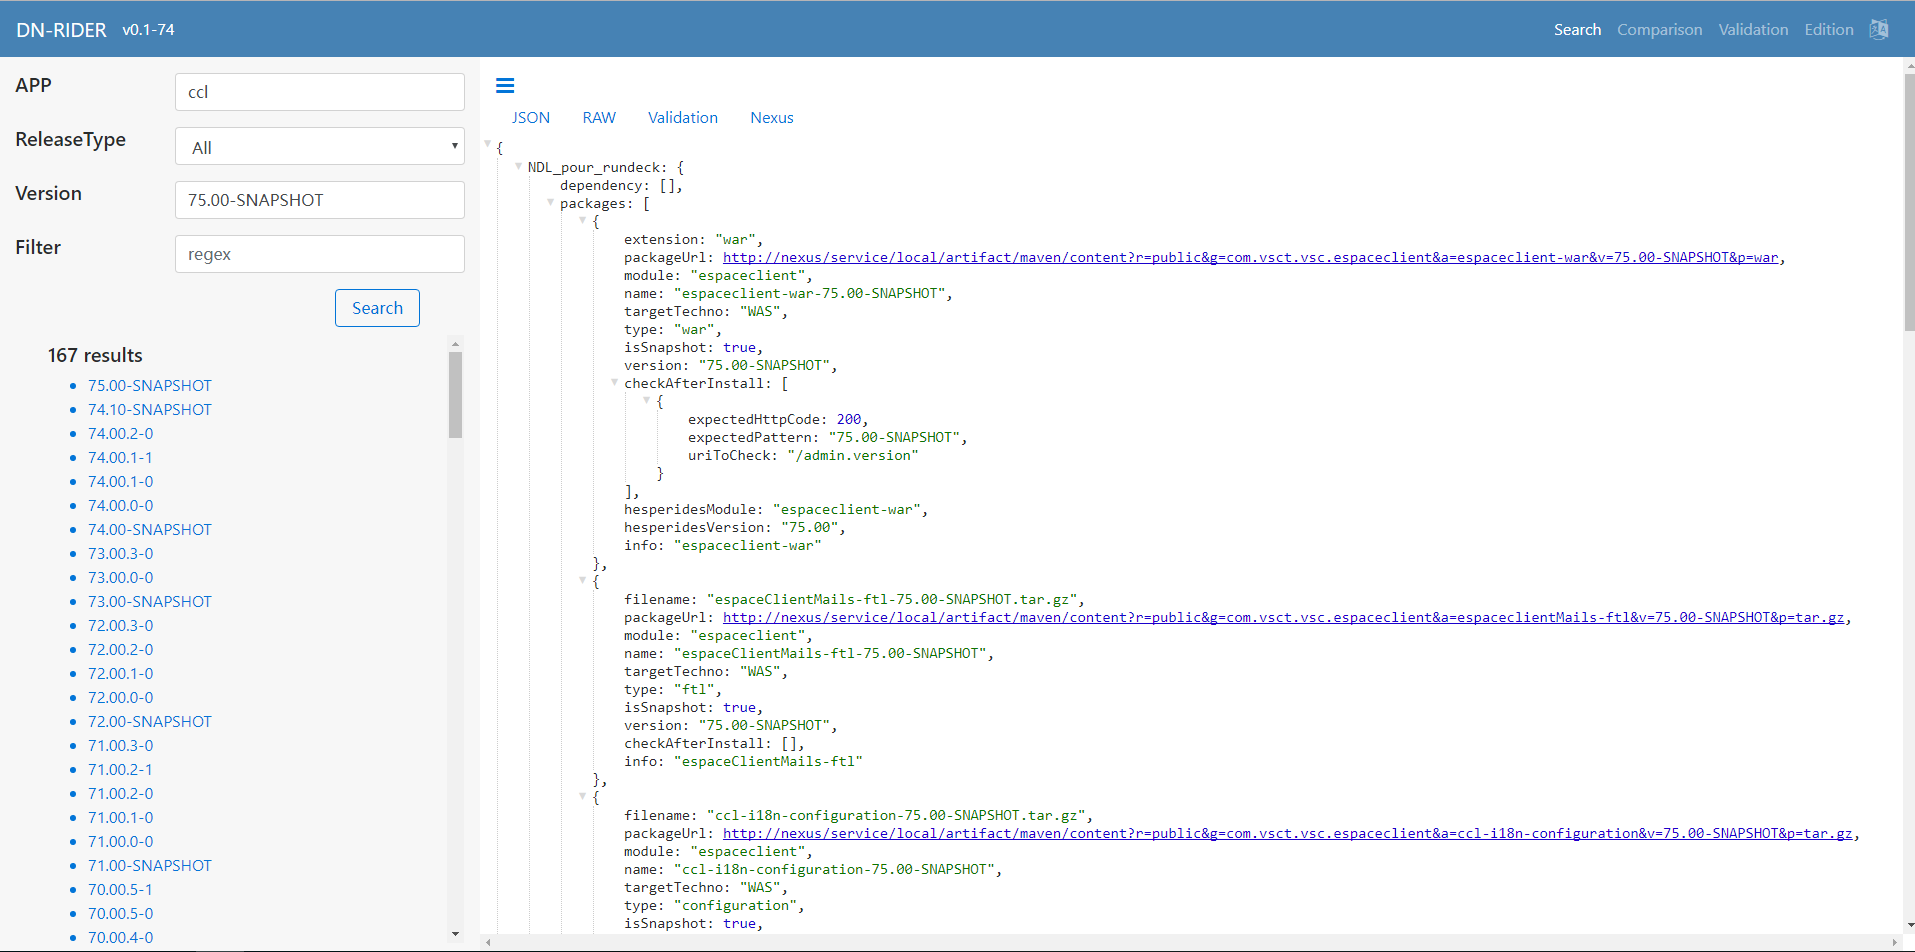
\includegraphics[width=0.8\textwidth]{page_search}
\caption{La page validation}
\label{fig:page_validation}
\end{figure}

\paragraph{La page edition(fig.\ref{fig:page_edition}): } Cette page contient des élements suivants:
\begin{itemize}
  \item Un sidebar collapsible qui contient un formulaire pour choisir les notes de livraisons;
  \item Une zone qui permet d'éditer une note de livraison;
  \item Une fênetre qui affiche les résultats de validation;
  \item Un modal(fig.\ref{fig:modal_save}) qui permet de stocker la note de livraison.
\end{itemize}

\begin{figure}[h]
\centering
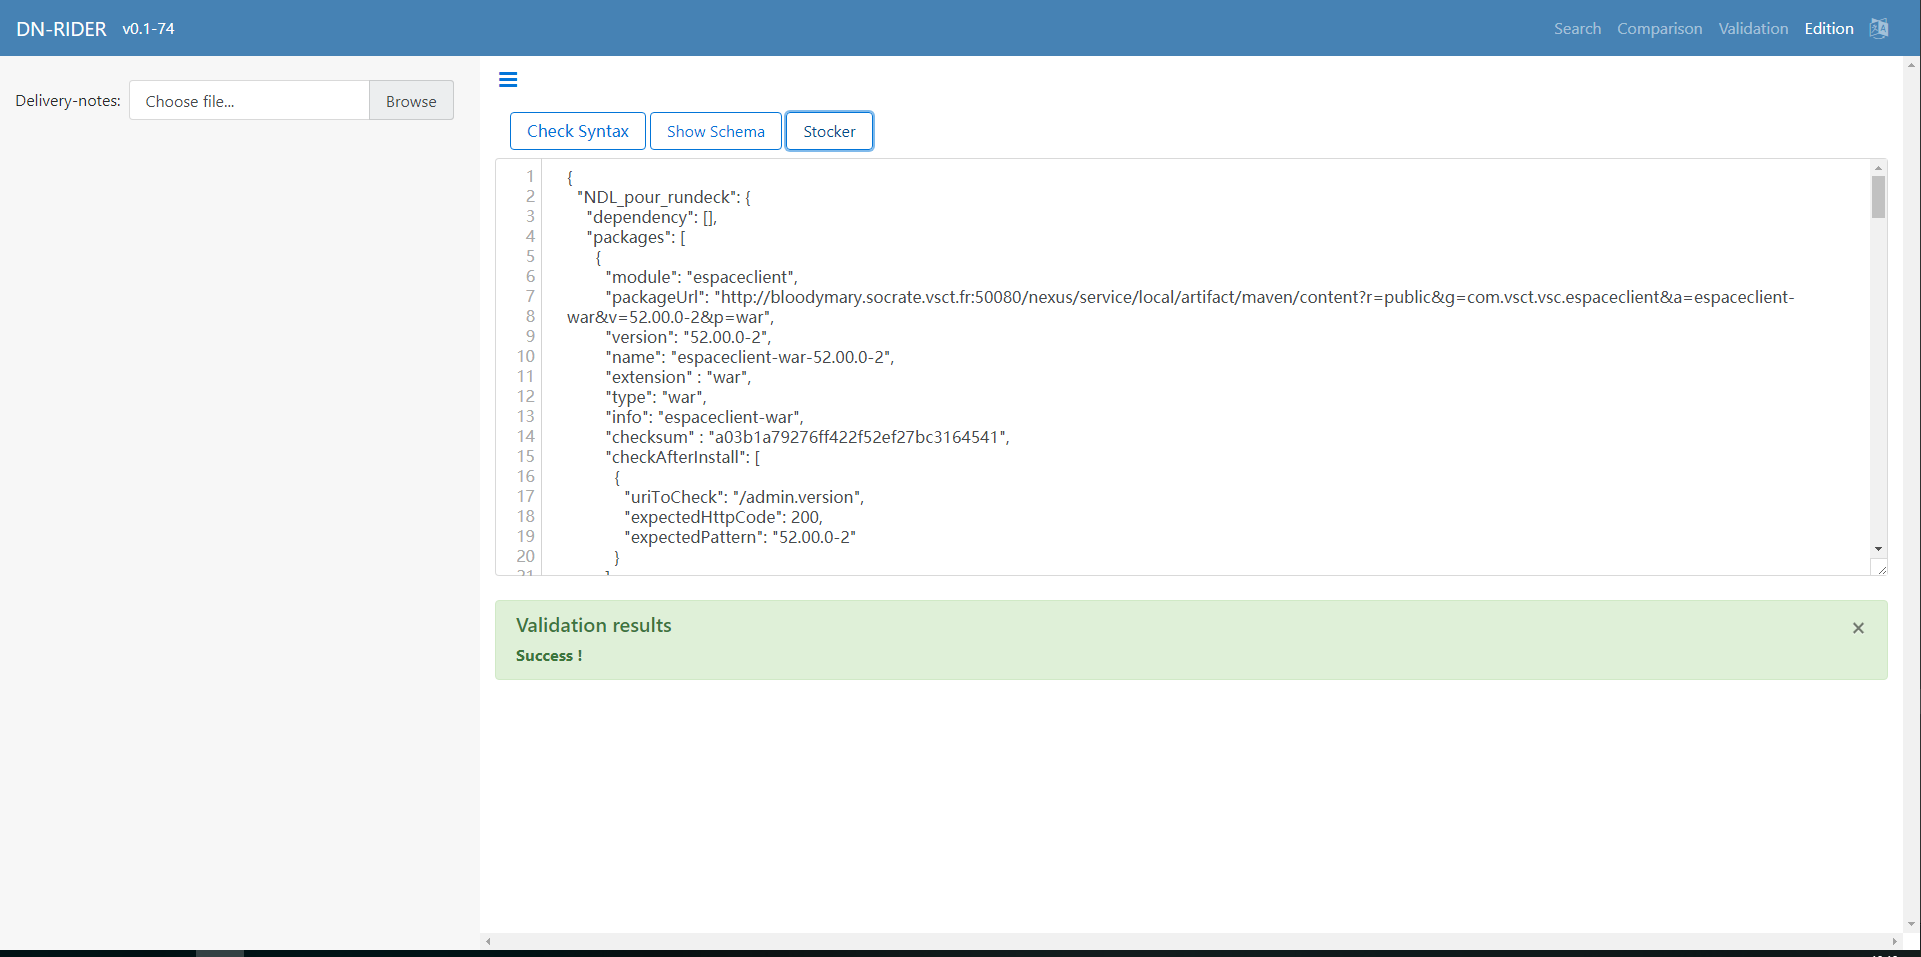
\includegraphics[width=0.8\textwidth]{page_edition}
\caption{La page edition}
\label{fig:page_edition}
\end{figure}

\begin{figure}[h]
\centering
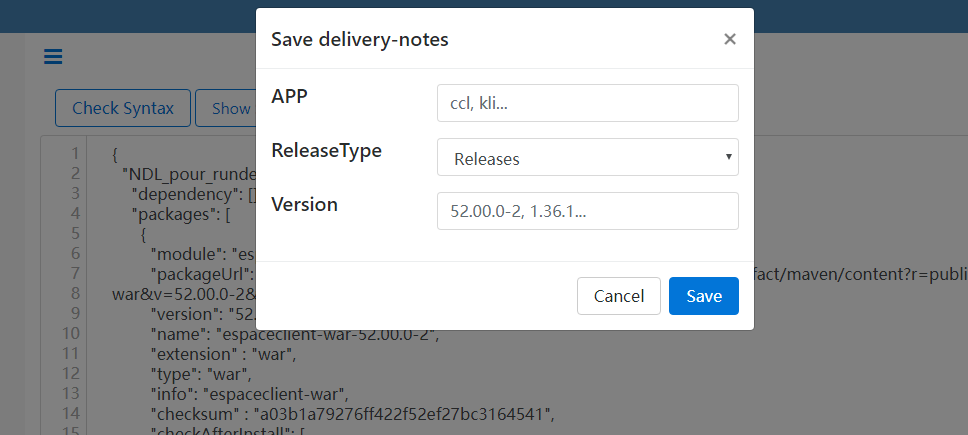
\includegraphics[width=0.6\textwidth]{modal_save}
\caption{Le modal configuration}
\label{fig:modal_save}
\end{figure}

\subsubsection{Api REST}

\paragraph{Api et swagger(fig.\ref{fig:page_swagger}):  } L'application fournie une interface api REST et une interface réalisé en Swagger pour la documentaion de l'api.

\begin{figure}[h]
\centering
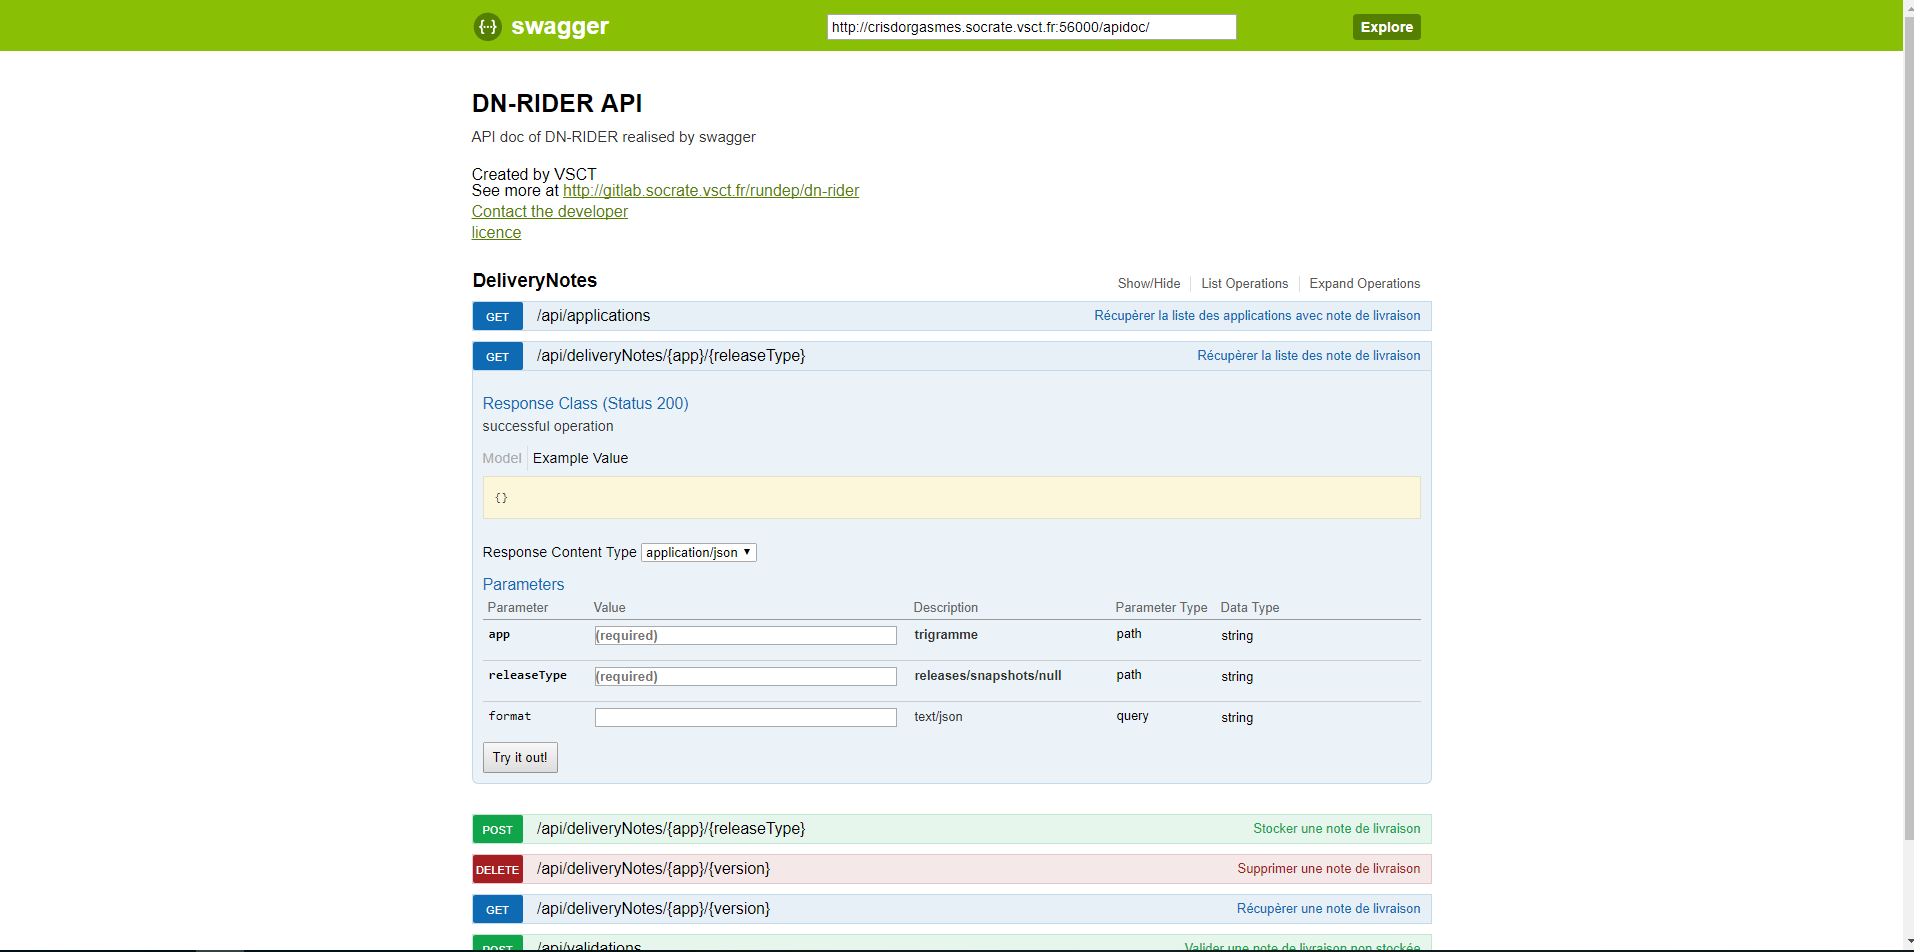
\includegraphics[width=0.8\textwidth]{page_swagger}
\caption{La page swagger}
\label{fig:page_swagger}
\end{figure}

\subsubsection{Continus Delivery(git, test unitaire, pipeline->deploiement auto)}

\subsection{Architecture}
\subsubsection*{Choix des technologies:}
\begin{itemize}
  \item Grails:
  Grails est un framework open source de développement agile d'applications web basé sur le langage Groovy et sur le patron de conception Modèle-Vue-Contrôleur.
  Il convient à la taille de ce project. En plus il y a référent compétent qui connait bien ce framework.
  \item Groovy:
  Groovy est le nom d'un langage de programmation orienté objet destiné à la plate-forme Java.
  Groovy utilise une syntaxe très proche de Java, par rapport à Java, il est moins verbeux et plus efficace.
  \item Bootstrap:
  Boostrap est un framwork front-end qui contient  une collection d'outils utile à la création du design de sites. C'est un ensemble qui contient des codes HTML et CSS, des formulaires, boutons, outils de navigation et autres éléments interactifs, ainsi que des extensions JavaScript en option. C'est l'un des projets les plus populaires sur la plate-forme de gestion de développement GitHub.
  Ca aide à créer l'IHM de site facilement.
  \item jQuery:
  jQuery est une bibliothèque JavaScript libre et multi-plateforme créée pour faciliter l'écriture de scripts côté client dans le code HTML des pages web.
   Etant donné la complécité de l'IHM de l'application, jQuery est suffisant pour réaliser les animations et les ajax.
  \item Backlog:
  Backlog se réfère à une accumulation d'œuvres en attente d'exécution ou aux commandes à remplir.
  Cette méthode convient à la méthode qu'on a appliqué au cours du project.
\end{itemize}


\subsubsection*{Architecture de l'application}
\paragraph{Modèle MVC :} L'application suit le motif Modèle-Vue-Contrôleur. Il est composé de  trois types de modules ayant trois responsabilités différentes : les modèles, les vues et les contrôleurs:
\begin{itemize}
  \item Modèle: Il n'y pas de base de donnée dans cette application. Ca correspont aux données de Nexus et à la cache.
  \item Vue: La présention de l'interface graphique. Realisé en utilisant Bootstrap et jQuery dans cette application.
  \item Contrôleur: La logique concernatn les actions effectuées par l'utilisateur. Réalisé en grails dans cette application.
\end{itemize}

\paragraph{La couche service:}
On extrait les codes techniques des controleurs et former des services, après on peut les appler depuis les controleurs. Ca aide à éviter les codes répétifs et rendre les codes métiers claire.
Par example, on crée une service "NexusConsumer" qui contient tous les opérations de Nexus.

\clearpage
